% 使用 ctex 文档类,支持中文
\documentclass[UTF8]{ctexart}

% 基础宏包
\usepackage{graphicx} % 调整图片
\usepackage{array}    % 增强表格功能
\usepackage{booktabs} % 绘制更美观的表格

% 文档开始
\begin{document}

\section{预测2028年首次获得奖牌的国家数量}
我们对2024年之前出现过的老项目,和2028年新增加的新项目分开讨论;老项目我们可以充分利用题目提供的数据,而对于2028年增加的5个新项目,我们通过查询权威资料来计算预测。

\subsection{老项目}
我们将国家分为两类:解体产生的国家,非解体产生的国家。因为我们统计发现,在1992年之后由于政治因素解体产生的新国家,会显著影响
首次获得奖牌的国家数量,因此我们必须对这两种国家分开讨论。
对2028年之前已经出现过的老项目,计算会有多少个非解体国家在这些老项目中第一次获得奖牌:
基于历史数据,我们的策略是结合ARIMA 模型 和 随机森林模型,利用时间序列数据和特征工程,生成预测结果及其置信区间。
模型适用的原因:奥运会首次获得奖牌的国家数量是典型的时间序列数据,具有潜在的趋势(参加国家数量增加,老项目数量增加等),并有四年一届的周期性,ARIMA模型可以很好捕捉到这些特性,来为2028年数据做预测;而随机森林模型能够捕捉到参加国家总数、奖牌总数等与首次获得奖牌的国家数量之间存在的复杂非线性关系,构建多棵决策树集成结果能够减少过拟合,并结合ARIMA模型得到的结果得到置信区间;前者捕捉时间序列线性依赖,而后者捕捉非线性依赖以及额外的特征。

我们将1896-2004年、2008-2024年划分为训练集和测试集,时间点为每届奥运会的年份,目标变量为首次获得奖牌的国家数量;对原始的目标变量做一阶差分和二阶差分,然后做ADF检验验证数据平稳性,结果如图所示原始序列的平稳性最好:
$\text{ADF Statistic}=-4.01,\text{p-value}=0.0014$

\begin{figure}[ht]
  \centering
  \begin{minipage}[b]{0.42\textwidth} % 第一张图片
    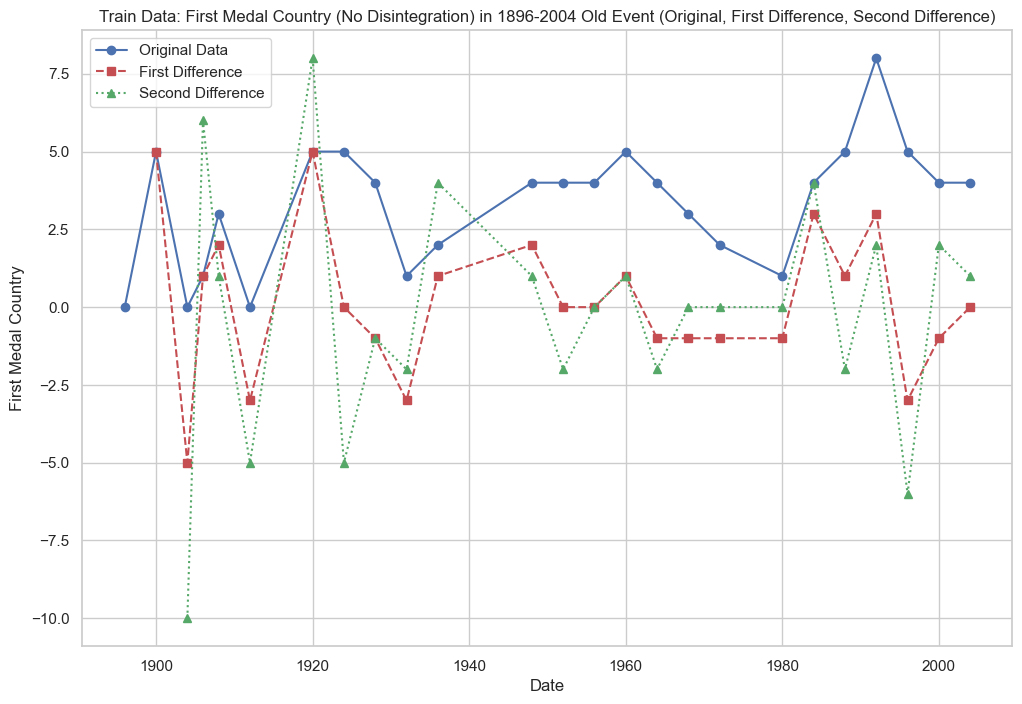
\includegraphics[width=\textwidth]{1} % 替换为你的图片文件名
    \caption{Origin Data,First Difference and Second Difference Trend Chart}
    \label{fig:image-a}
  \end{minipage}
  \hfill % 增加水平间距
  \begin{minipage}[b]{0.42\textwidth} % 第二张图片
    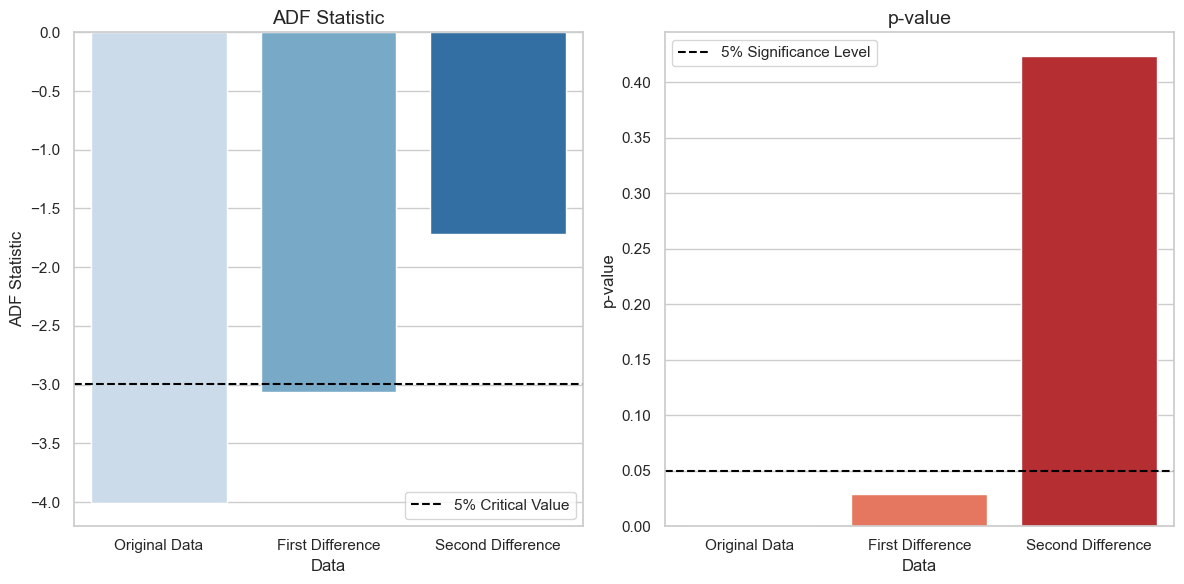
\includegraphics[width=\textwidth]{2} % 替换为你的图片文件名
    \caption{ADF Statistic and p-value}
    \label{fig:image-b}
  \end{minipage}
  %\caption{Stationarity Test}
  \label{fig:images}
\end{figure}

绘制原始序列的ACF与PACF图像($
\operatorname{ACF}(k)=\rho_{\mathrm{k}}=\frac{\operatorname{Cov}\left(\mathrm{y}_{\mathrm{t}}, \mathrm{y}_{\mathrm{t}-\mathrm{k}}\right)}{\operatorname{Var}\left(y_t\right)}
$,$\operatorname{PACF}(k)=\frac{\operatorname{cov}\left[\left(z_t-\bar{z}_t\right),\left(z_{t-k}-\bar{z}_{t-k}\right)\right]}{\sqrt{\operatorname{var}\left(Z_t-\bar{z}_t\right)} \sqrt{\operatorname{var}\left(Z_{t-k}-\bar{z}_{t-k}\right)}}$),
都是拖尾,可以选取ARIMA模型;使用AIC准则确定ARIMA模型的参数,其中$AIC=2K-2ln(L)$,$k$是模型参数个数,$L$是模型最大似然值。画出热力图可视化,当$p=0,q=2$时,AIC有最小值;因此我们选择ARIMA(0,0,2)作为最优模型。
\begin{figure}[ht]
  \centering
  \begin{minipage}[b]{0.42\textwidth} % 第一张图片
    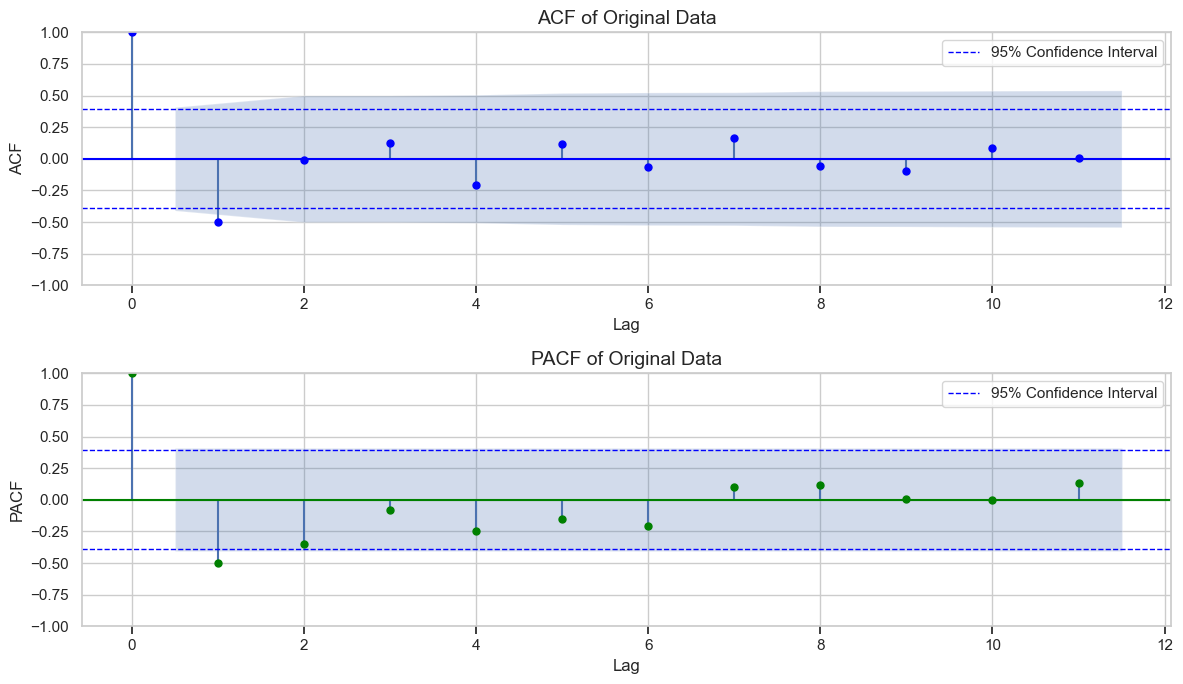
\includegraphics[width=\textwidth]{3} % 替换为你的图片文件名
    \caption{Second Difference AFC and PAFC}
    \label{fig:image-a}
  \end{minipage}
  \hfill % 增加水平间距
  \begin{minipage}[b]{0.42\textwidth} % 第二张图片
    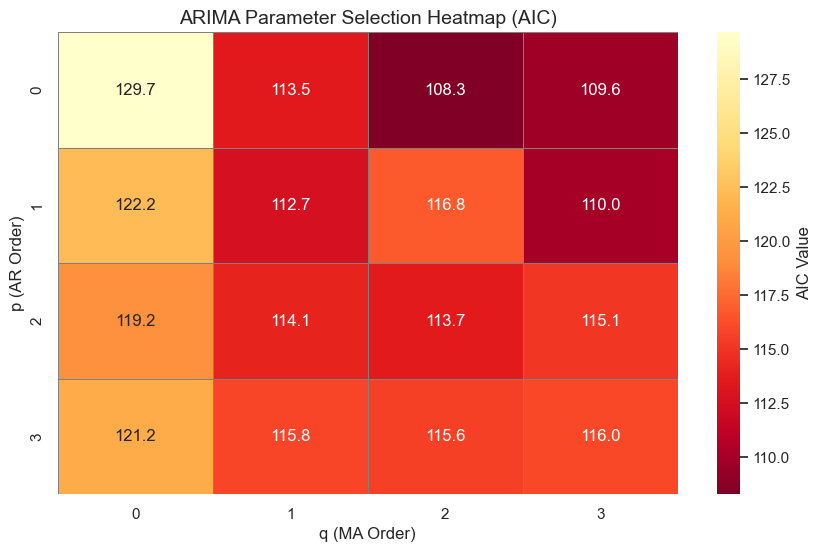
\includegraphics[width=\textwidth]{4} % 替换为你的图片文件名
    \caption{AIC Heatmap}
    \label{fig:image-b}
  \end{minipage}
  \label{fig:images}
\end{figure}


为了验证 ARIMA 模型的拟合效果,我们对模型残差进行了以下检验。首先,绘制残差的 \textbf{ACF} 和 \textbf{PACF} 图,并利用 \textbf{Ljung-Box 检验} 评估残差的自相关性,结果表明残差在选定滞后阶数内无显著自相关性($p > 0.05$)。其次,通过绘制残差的 \textbf{直方图} 和 \textbf{QQ 图},并结合 \textbf{Shapiro-Wilk 检验},验证残差近似服从正态分布($p > 0.05$)。此外,通过计算 QQ 图的拟合直线斜率和误差,进一步确认残差的正态性。综上所述,残差无明显自相关性且近似服从正态分布,表明 ARIMA 模型拟合效果良好,满足建模假设。

\begin{figure}[ht]
  \centering
  \begin{minipage}[b]{0.42\textwidth} % 第一张图片
    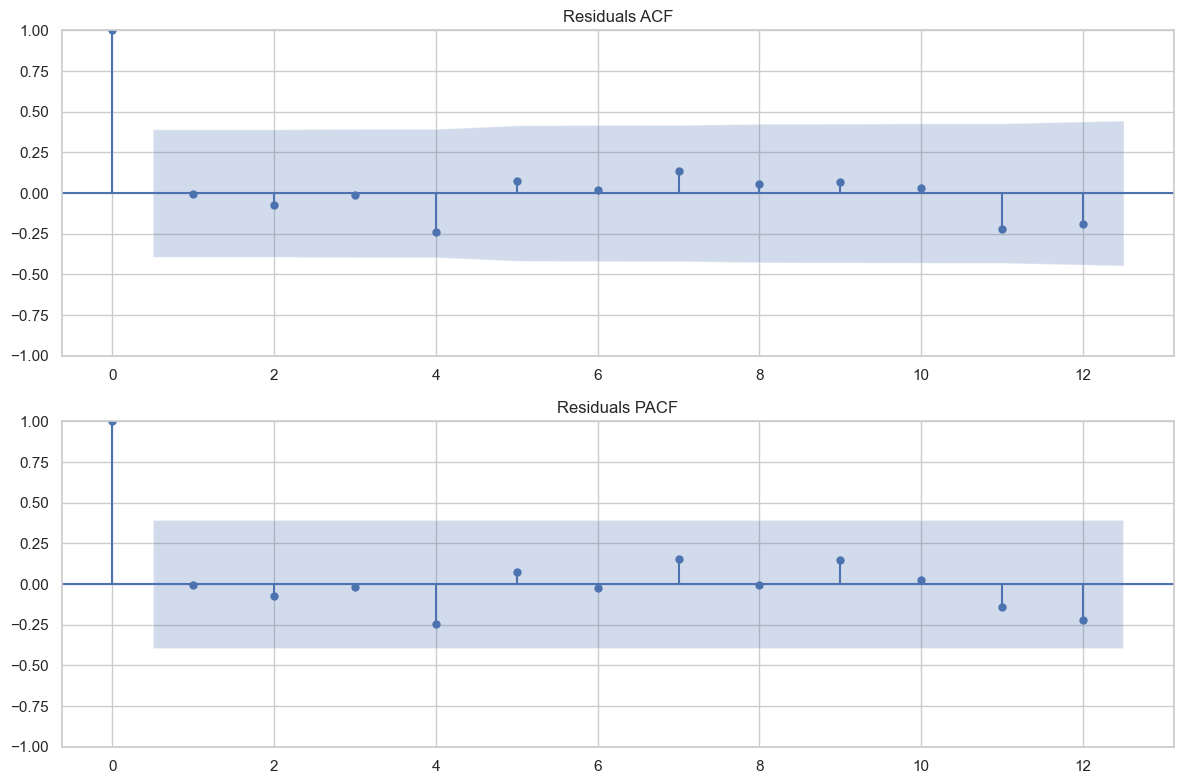
\includegraphics[width=\textwidth]{5} % 替换为你的图片文件名
    \caption{Residuals ACF and Residuals PACF}
    \label{fig:image-a}
  \end{minipage}
  
  \begin{minipage}[b]{0.42\textwidth} % 第一张图片
    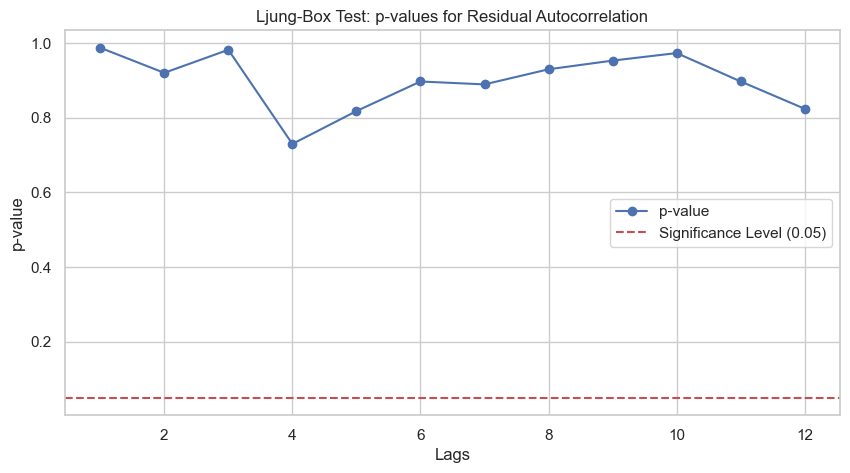
\includegraphics[width=\textwidth]{8} % 替换为你的图片文件名
    \caption{Ljung-Box Test}
    \label{fig:image-a}
  \end{minipage}
  
  \begin{minipage}[b]{0.42\textwidth} % 第二张图片
    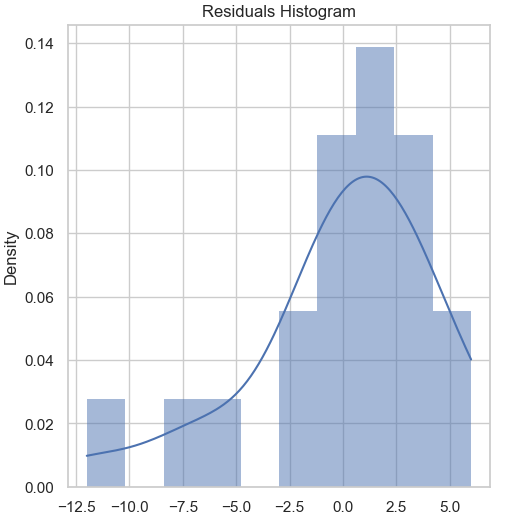
\includegraphics[width=\textwidth]{6} % 替换为你的图片文件名
    \caption{Shapiro-Wilk Test}
    \label{fig:image-b}
  \end{minipage}
  
  \label{fig:images}
  \begin{minipage}[b]{0.42\textwidth} % 第二张图片
    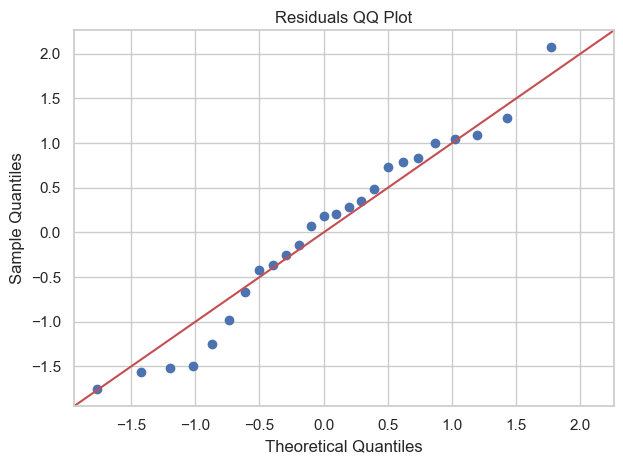
\includegraphics[width=\textwidth]{7} % 替换为你的图片文件名
    \caption{Residuals QQ Plot}
    \label{fig:image-b}
  \end{minipage}
  
  \label{fig:images}
\end{figure}

然后我们用得到的ARIMA模型对2028年首次获得奖牌的国家数量进行预测,预测值为3.09;将这个预测值和此前的训练集作为特征带入到随机森林模型中进行训练,得到
2028年首次获得奖牌的国家数量的95\%置信区间为$[2.58,4.87]$:
\begin{figure}[ht]
  \centering
  \begin{minipage}[b]{0.42\textwidth} % 第一张图片
    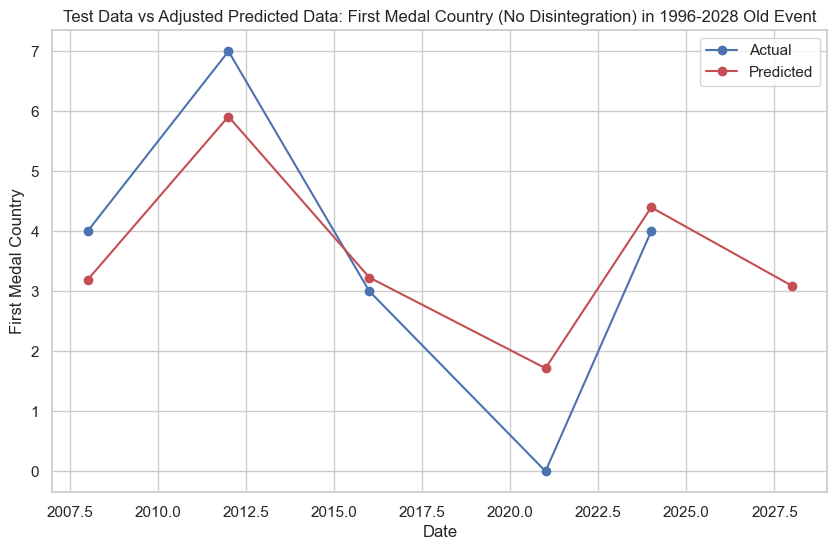
\includegraphics[width=\textwidth]{9} % 替换为你的图片文件名
    \caption{Actual vs Predicted First Medal Countries(No Disintegration) (2008-2028)}
    \label{fig:image-a}
  \end{minipage}
  
  \begin{minipage}[b]{0.42\textwidth} % 第一张图片
    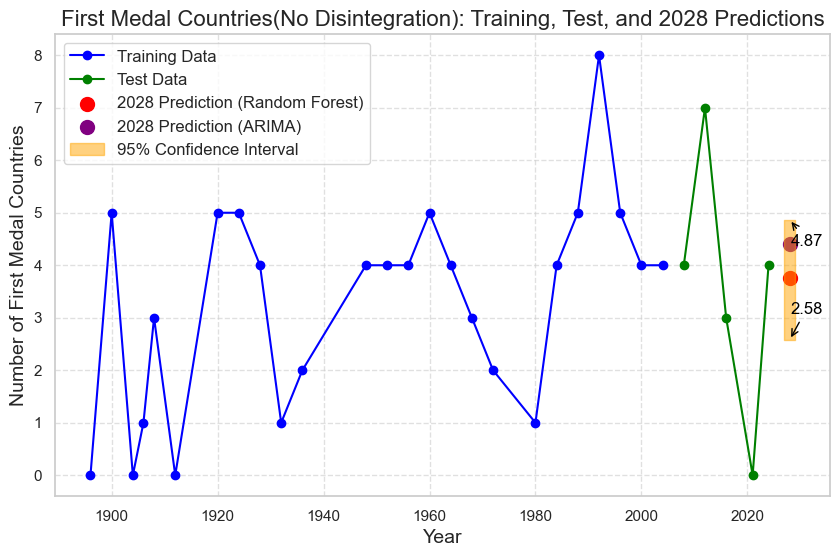
\includegraphics[width=\textwidth]{10} % 替换为你的图片文件名
    \caption{First Medal Countries(No Disintegration): Training, Test, and 2028 95\% Confidence Interval Prediction}
    \label{fig:image-a}
  \end{minipage}
\end{figure}

然后计算多少个解体产生的国家在老项目中首次获得奖牌,统计1996-2024年解体产生国家数据,原始数据、一阶差分、二阶差分均未能通过平稳性测试,根据这个数据直观特征,我们使用指数回归模型进行拟合,预测得到2028年解体产生国家首次获得奖牌的数量及置信区间,可以认为是0.

\begin{figure}[h!]
    \centering
    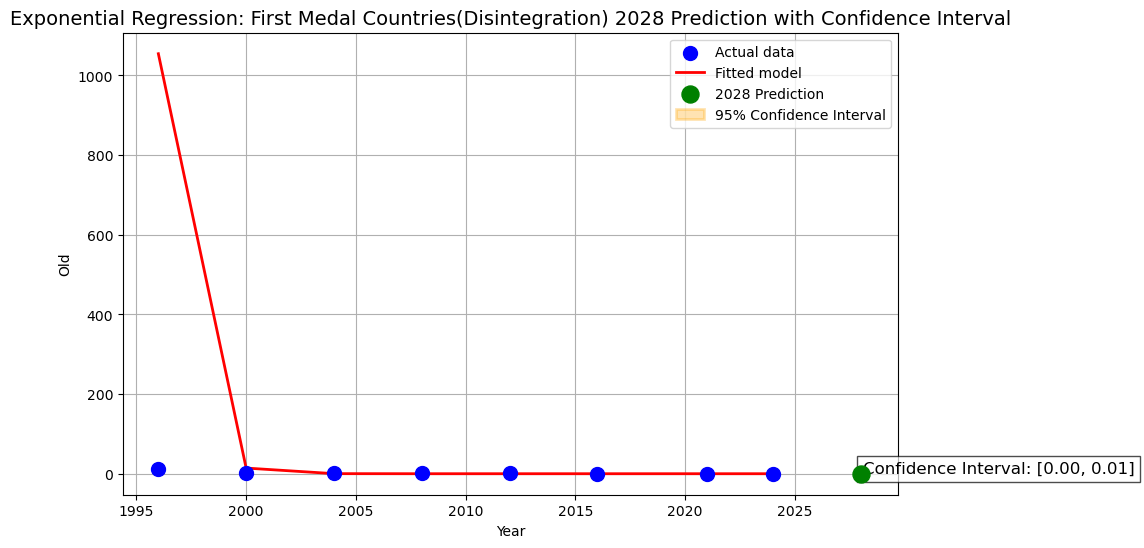
\includegraphics[width=0.5\textwidth]{jieti}  % 调整为50%的宽度,您可以根据需要调整
    \caption{Exponential Regression Model:First Medal Country(Disintegration) 2028 95\% Confidence Interval Prediction}
    \label{fig:sample-image}
\end{figure}

\end{document}